
\part{Introducing Reflex}
\chapter{Background}
Recently there has been a significant move to create languages that run on top of the Java Virtual Machine. These languages are usually integrated as a fundamental "Java Scripting Language" - such as JRuby \index{JRuby} (an implementation of Ruby \index{Ruby}), Jython \index{Jython} (the equivalent of Python \index{Python}) and Rhino \index{Rhino} (a JavaScript \index{JavaScript} implementation) or as a fully defined language that hooks into the JVM at a lower level. Examples of these languages would include Clojure \index{Clojure} (a functional Lisp dialect), Groovy \index{Groovy} (a scripting language) and Scala \index{Scala} (an object-oriented and functional programming language). 

\Reflex is a procedural language that hooks into the JVM at a lower level. Its syntax is similar to Python (without the indentation) and there are a number of built-in functions and special operators that are semantic short cuts when interacting with \Rapture.

This book provides a detailed description of \Reflex.

\section{Why Reflex?}
The designers of \Rapture felt that it was very important to provide a non-compiled way of running programs "in the cloud"\index{cloud}. The idea was that \Rapture application developers could define a lot of their data manipulations in a scripting language and then have \Rapture run these "programs" on the servers that make up an installed system. If such a program could be agnostic to the machine (actual server) it was running on such manipulations could be run in a scalable way across all of the servers that make up a \Rapture system.

Initially the support for such a scripting language was built using JRuby and Jython - two well established languages that have a well educated developer base. Unfortunately this support ended up being impractical - both from a licensing perspective and from the fact that the scripting environment for these languages was very resource (time and memory) intensive. For these reasons it was decided to create a small language (now called \Reflex) to provide the "glue" for the data interactions in \Rapture.

\section{A short summary of Rapture}
\Rapture is a system for storing and manipulating data in a cloud (or distributed) server environment. Data is usually stored in "documents" \index{document} in a json \index{json} format and \Rapture isolates a developer from the underlying technology used to store that data. When data is changed in \Rapture scripts can be run to act upon that change. \Rapture also defines the concept of a workflow \index{workflow} - a set of tasks that are executed serially to perform a formal update to the data (such as an End Of Day process). Each step in a workflow is implemented by the execution of a script. \Rapture has a rich API that is exposed through a HTTP based protocol. Client side implementations of this API have been created for Python, Ruby, Java, .NET \index{.NET} (and VBA \index{VBA} for Excel \index{Excel} spreadsheets) and JavaScript\index{JavaScript}. There is also a REST \index{REST} based interface for even easier to access the documents that make up a \Rapture system in a RESTful way. \Rapture has a full entitlements \index{security} system to protect from unauthorized activity and a full audit trail to record authorized activity. \Rapture is also customized through many hook mechanisms - to provide analytics in a Risk Management System or to provide market data for pricing. The book "\Rapture in Action" describes this environment in full detail. The important thing to understand is that a scripting language "binds" the \Rapture system together - it is the glue that runs the workflow system, it is used to propagate events and it can be compared to the "stored procedure language" of a "database management system". 

\chapter{Server hosted scripting}
The initial use for \Reflex was to provide a scripting language that could be run on a server. However the same language could also be used to help setup a \Rapture system and hooks were also built in to handle file based io - something that normally would be restricted on a cloud/distributed server environment. In fact a \Reflex environment now has a number of "hooks" that can be implemented (or wired) differently depending on the context. In general the environment looks like the logical diagram below.

\begin{figure}[H]
\centering
\begin{tikzpicture}
\node[external](Reflex) { \Reflex     };
\node[api] (File) [below right=of Reflex] { File IO }
   edge [post, bend right=45] (Reflex);
\node[client] (Plugin) [right=of Reflex] { Plugins}
   edge [post] (Reflex);
\node[api] (API) [below left=of Reflex] { \Rapture }
   edge [post,bend left=45]  (Reflex);
\node[api] (Scripting) [below=of Reflex] { Scripting }
   edge [post] (Reflex);
\node[api](Debugger) [above left=of Reflex] { Debugger }
   edge [post, bend left=45] (Reflex);
\end{tikzpicture}
\caption { Logical \Reflex environment }
\end{figure}

Here we see that \Reflex can reach out to a debugger, a \Rapture environment (for calling its API), a Scripting environment (for loading other scripts) and an IO sub-system for loading and saving data to a file system.

When running within a \Rapture server, the implementations are frozen to protect the environment:

\begin{figure}[H]
\centering
\begin{tikzpicture}
\node[external](Reflex) { \Reflex     };
\node[internal] (File) [below right=of Reflex] { Disabled }
   edge [post, bend right=45] (Reflex);
\node[client] (Plugin) [right=of Reflex] { Plugins}
   edge [post] (Reflex);
\node[api] (API) [below left=of Reflex] { \Rapture }
   edge [post,bend left=45]  (Reflex);
\node[api] (Scripting) [below=of Reflex] { Scripting }
   edge [post] (Reflex);
\node[internal](Debugger) [above left=of Reflex] { Disabled }
   edge [post, bend left=45] (Reflex);
\end{tikzpicture}
\caption { Server \Reflex environment }
\end{figure}

Here the debugger and the file/IO subsystems are disabled.

\Reflex can also be run on a local desktop, or on a server outside of a \Rapture environment. In this case the bindings of the environment are as below:
\begin{figure}[H]
\centering
\begin{tikzpicture}
\node[external](Reflex) { \Reflex     };
\node[api] (File) [below right=of Reflex] { File }
   edge [post, bend right=45] (Reflex);
\node[client] (Plugin) [right=of Reflex] { Plugins}
   edge [post] (Reflex);
\node[api] (API) [below left=of Reflex] { \Rapture }
   edge [post,bend left=45]  (Reflex);
\node[api] (Scripting) [below=of Reflex] { Scripting }
   edge [post] (Reflex);
\node[api](Debugger) [above left=of Reflex] { Debugger }
   edge [post, bend left=45] (Reflex);
\node[external](HTTP) [below left=of API] { HTTP }
   edge [post] (API)
   edge [post] (Scripting);
\node[ewd](Remote) [below=of HTTP] { Remote\nodepart{second}\Rapture }
   edge [post] (HTTP);
\end{tikzpicture}
\caption { External \Reflex environment }
\end{figure}

In this case the environment has a \Rapture system wired in via a standard HTTP based API - all \Rapture commands in \Reflex will still work through that API. In a server based environment the security context is set by \Rapture (and is based on the ultimate initiator of the \Reflex process). In the external approach the user security context is set either by using a \Rapture "API key" or by logging in manually through the Reflex runner application.

\section{Installing Reflex}
There are three options for using \Reflex. The most common use for \Reflex is to run scripts from within a \Rapture environment - you upload scripts to \Rapture and then call them through either \Rapture's API call \verb+runProgram+ or through a \Rapture workflow, operation or event handling. For testing and debugging it is preferable to install a local environment to play with. This section describes how to do that.

\Reflex is bundled into an application called \emph{ReflexRunner} that can be used to run \Reflex scripts. ReflexRunner is a command line java application that can be downloaded from the \href{http://incapture.github.com/RaptureRepo/release}{\Rapture Release Site}. Once downloaded it can be run using java as follows:

\begin{verbatim}
java -jar [ReflexRunner.jar] 
          -r [RaptureAPIURL] -f [ReflextScript]
\end{verbatim}

Optional parameters are listed below:

\begin{verbatim}
-u 'user' - User name to login as
-p 'password' - Password to use
-d - Start debugger
\end{verbatim}

\section{Installing into Eclipse}
\Reflex (and \Rapture) have an Eclipse plugin that can also be used to assist in the development of \Reflex scripts. This section describes how to install the plugin.

The first step is to install the latest version of Eclipse (recommended is at least the Java IDE for Eclipse) from \url{http://eclipse.org}.

From within Eclipse, navigate to the Help menu and click on \emph{Install New Software...}. You should see a dialog similar to that in Figure~\vref{fig:HelpInstall}.

\begin{figure}[htb]
\centering
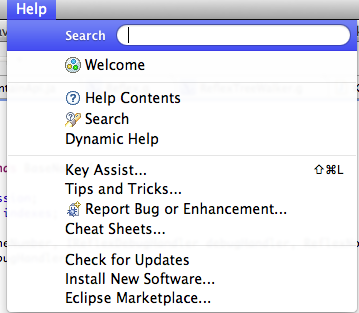
\includegraphics[scale=0.5]{images/HelpInstall.png}
\caption{Help/Install menu in Eclipse}
\label{fig:HelpInstall}
\end{figure}

In the Install dialog, click on the Add button and then add the Incapture \Rapture Eclipse site to the Eclipse sites. If you have already done this simply pick that site from the drop-down instead. This is shown in Figure~\vref{fig:InstallDialog}.

\begin{figure}[htb]
\centering
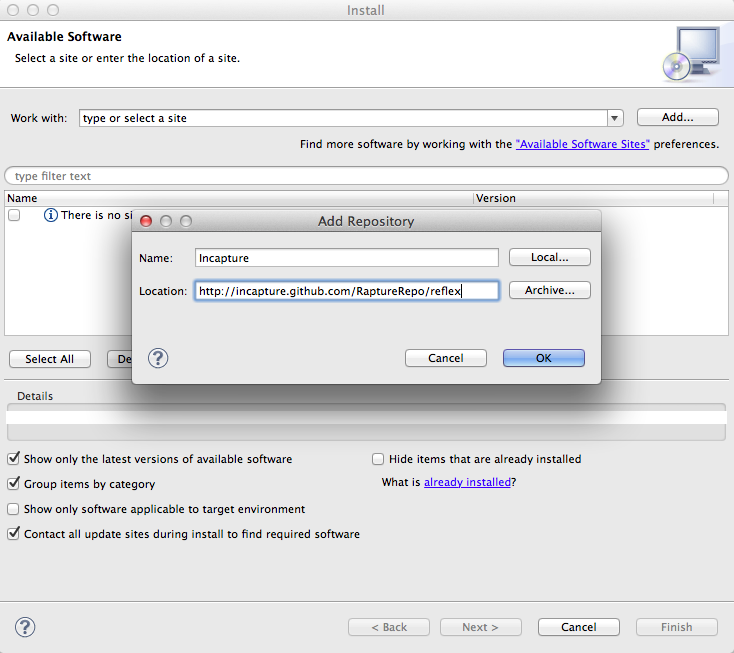
\includegraphics[scale=0.5]{images/InstallDialog.png}
\caption{Install Dialog in Eclipse}
\label{fig:InstallDialog}
\end{figure}

Clicking on OK will add the site and determine what updates or options are available. In this case pick Rapture and if more than one item is shown pick the item with the greatest release version. The dialog will look similar to that in Figure~\vref{fig:AvailableSoftware}.

\begin{figure}[htb]
\centering
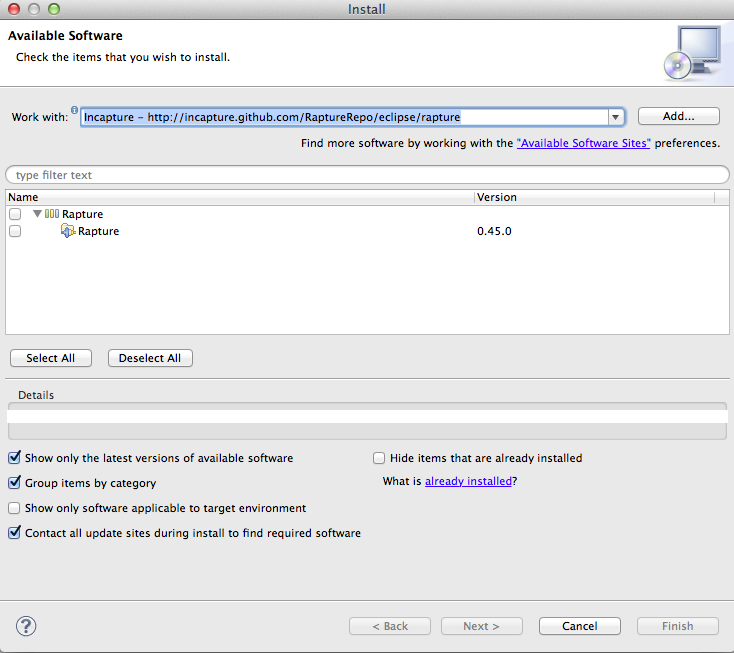
\includegraphics[scale=0.5]{images/AvailableSoftware.png}
\caption{Available Software}
\label{fig:AvailableSoftware}
\end{figure}

Clicking Next will then go through a validation process and eventually you will need to accept the license agreement and then restart Eclipse using a dialog similar to that in Figure~\vref{fig:License}.

\begin{figure}[htb]
\centering
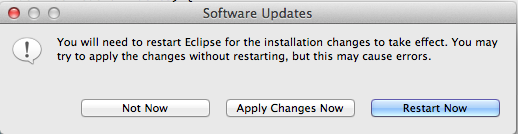
\includegraphics[scale=0.5]{images/AcceptLicense.png}
\caption{Accept License}
\label{fig:License}
\end{figure}

\section{Configuration}

The first thing to do post-install is to configure the \Rapture plugin for your local environment. The plugin will need to be told the location of the \Rapture environment you will be connecting to. You do this in the Preferences dialog of Eclipse, in the \Rapture section as shown in Figure~\vref{fig:Configuration}.

\begin{figure}[htb]
\centering
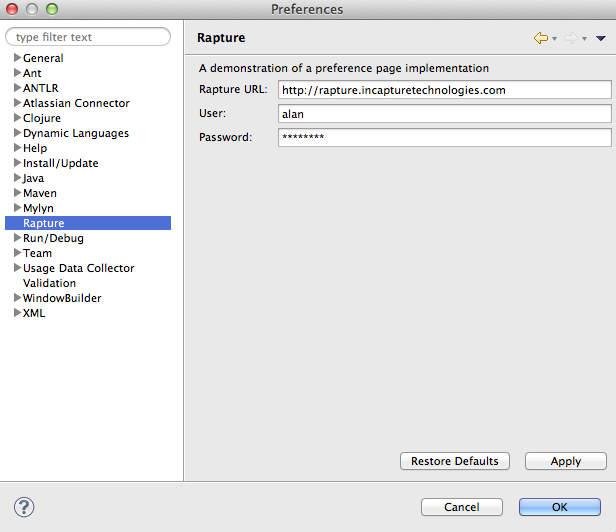
\includegraphics[scale=0.5]{images/Configuration.png}
\caption{Configuration Dialog}
\label{fig:Configuration}
\end{figure}

\section{Reflex scripts}
(Script running, Console output, Debug output, Caveats)

\section{Reflex fundamentals}
\Reflex is a basic procedural language with a few special operators \index{operator} and built-in functions \index{function} to make \Rapture interactions quicker to write. In this case the meaning of "procedural" is simply that in \Reflex you can define functions and invoke those functions. This section describes the fundamental characteristics of the language.
\section{Hello, World}
The simplest program in \Reflex uses the built-in function \verb+println+ \index{println} to print out the contents to standard out:
\begin{lstlisting}[caption={Hello world}]
// This is Hello World in Reflex
println('Hello, world');

\end{lstlisting}

Running the above program in Eclipse or through the ReflexRunner will print out the string 'Hello, world' on the console. It introduces two concepts. Line 1 shows how comments are defined in \Reflex. Comments are prefixed with a double slash and continue to the end of the line. This is the only comment style in \Reflex. Line 2 shows the built-in function \verb+println+ and the fact that strings can be enclosed either in single quotes or double quotes. Finally statements in \Reflex are terminated by semi-colons.

\section{Variables and Types}

Variables \index{variable} in \Reflex are created upon first declaration and can be named using the letters of the alphabet and the digits 0 - 9. Some examples of variable names are shown in the table below:

\begin{table}[h]
\centering
\begin{tabular} { | l | l | }
Variable Name & Valid? \\
\hline
abc & Yes \\
aB0 & Yes \\
a*3 & No (contains a *) \\
reflex & Yes \\
\_var & No (contains a \_) \\
\end{tabular}
\caption{Variable names in \Reflex}
\end{table}

Types \index{type} in \Reflex are inferred from the context in which a value is assigned, and wherever possible a type will be coerced into another if the other type is needed for a context. The types are listed in table \vref{tab:Types}.

\begin{table}[h!]
\centering
\begin{tabular} { | c | c | p{5cm} | }
\hline
Type & Example & Description \\
\hline
string & 'Hello' & A string, an array of characters \\
number & 4.0 & A number, either an integer or a float, depending on context \\
boolean & true & A boolean value, either true or false \\
list & \verb+[ 1, 2, 3]+ & A list of values \\
map & \verb+{ 'key' : 'value' }+ & An associate map, mapping keys (strings) to values. \\
date & \verb+ date() + & A date. \\
time & \verb+ time() + & A time. \\
file & \verb+ file('test.txt') + & A file object, used to read or write data. \\
queue & \verb+ que('test','thequeue')+ & A queue object, used to receive and send messages in \Rapture.\\
nul & \verb+ null + & An object representing a nul value.\\
void & \verb+ void + & An object representing "no" object.\\
\hline
\end{tabular}
\label{tab:Types}
\caption{Types in \Reflex}
\end{table}

The more complex types (queue, file) will be introduced in a later section on integration with \Rapture.

\section{Type conversion}
\Reflex will attempt to convert \index{conversion} from one type to another as needed. The table below shows what conversions are implicit and which ones need a little help from a built in function.

\begin{table}[h!]
\centering
\begin{tabular} { | c | c | c | c | c | c | c | c |}
\hline
       & \multicolumn{7}{c|} {From} \\ \hline
To     & String & Number & Boolean & List & Map & Date & Time\\
\hline
String &        &  auto  &  auto   & auto & auto & auto & auto\\
Number &  cast  &        &  n/a    &  n/a & n/a & Julian & Millis\\
Boolean&  n/a   &  n/a   &         & n/a  & n/a & n/a & n/a \\
List   &  n/a   &  n/a   &  n/a    &      & n/a & n/a & n/a \\
Map    &  n/a   &  n/a   &  n/a    & n/a  & n/a & n/a & n/a  \\
Date   &  YYYYMMDD & Julian  & n/a & n/a & n/a & & n/a \\
Time   &  HH:MM:SS & Millis & n/a & n/a & n/a & n/a & \\
\hline
\end{tabular}
\caption{Conversions in \Reflex}
\end{table}

\section{Initialization}
\index{initialize}\Reflex types are determined by context - for example the result of calling the built-in \verb+size+ function is a number, so assigning a variable to the result of calling that function will result in a numeric variable being created. Another way of defining the type of a variable is to initialize it. Reflex uses the format of the initialization to determine the type.

A variable initialization can also be prefixed with the keyword \verb+const+\index{const}. This keyword ensures that the value of this variable will be unchanged after first assignment, and that the variable will be accessible globally, including within functions.

\subsection{String}
The string type is initialized through a statement enclosed in either single quotes or double quotes. The different quoting options are equivalent in \Reflex - the choice is a matter of convenience. If your string needs to contain double quotes you can enclose it in single quotes and vice versa.\index{quote}
\begin{lstlisting}[caption={String initialization}]
// String initialization
a = 'a string';
b = 'another string';
c = "A string in quotes";
const d = "There's a string in here somewhere";
\end{lstlisting}

\subsection{Number}
The number \index{number} type is initialized through a statement that represents a number - either an integer (a series of digits) or a floating point number through either a series of digits, a decimal point and a further series of digits, or through the definition of a number through scientific notation. If you suffix a number representation with a capital L the number will be locked to an internal integer \index{integer} type, which is useful when using these numbers in native Java calls.
\begin{lstlisting}[caption={Number initialization}]
// Number initializaion
a = 10;
b = 100.4;
const c = 5L;
d = 4.5E04; // equivalent to 45000
\end{lstlisting}
\subsection{Boolean}
The boolean \index{boolean} type is defined using the keywords \verb+true+ and \verb+false+, and of course can be initialized through the use of a boolean statement (see boolean operators in a later section).
\begin{lstlisting}[caption={Boolean initialization}]
// Boolean initialization
a = true;
const b = false;
c = (1 == 1); // c == true
\end{lstlisting}
\subsection{List}
The list \index{list} type is defined using square brackets, with elements of the list being separated by commas. The elements can be any expression which includes the name of an existing (pre-defined) variable.
\begin{lstlisting}[caption={List initialization}]
// List initialization
a = []; // An empty list
const b = [1, 2, 3, 4, 5]; 
c = ['A string', 1, []]; // A list of a string, a number, and an empty list
\end{lstlisting}
\subsection{Map}
A map \index{map} is initialized using a JSON style format and is best demonstrated through example.
\begin{lstlisting}[caption={Map initialization}]
// Map initialization
a = {}; // An empty map
b = { 'a' : 4 }; // A map containing a 
                 // single entry, with 
                 // the key 'a' and the value 4
c = { 'one' : 1, 'two' : 2, 'three' : 3 };
const d = { 'outer' : { 'inner' : true }};
\end{lstlisting}
\section{Simple examples}
Based on our understanding of types and variables, and our simple \verb+println+ function, we can create some new \Reflex scripts. Here is a longer script that creates some variables and introduces some of the operators that will be expanded upon in the next section.

\begin{lstlisting}[caption={Variables and Types}]

// An example Reflex script showing variables and types
x = 10;
y = "Hello";
z = x + 1;
println("Z is " + z);
\end{lstlisting}

In this example we have defined three variables, $x$, $y$ and $z$. $x$ and $z$ are ultimately numbers and $y$ is a string. We create the variable $x$ on line 3, and $y$ on line 4. $z$ is implicitly created as the value of $x+1$ (i.e. 11). Finally we print out the value of $z$ on line 6, but note that we have used the $+$ operator on a string (\verb+Z is+) and a number (the variable $z$). In this case \Reflex will convert $z$ from a number to a string and then append the strings together.

\chapter{Operators}
Operators \index{operator} in \Reflex will, in the most part, be very familiar to developers of other languages. There are boolean \index{boolean} operators ($==$, $>=$, $<=$, $<$, $>$, $!=$, $||$, $\&\&$), arithmetic \index{arithmetic} operators ($+$,$-$,$/$,$*$,$\%$) and index \index{index} operators (\verb+[ ]+). The ternary \index{ternary} operator $?$ is also supported. The use of these \emph{simple} operators is best illustrated by example. The examples below also introduce the \verb+assert+ built-in function - it aborts the \Reflex script with an error if the result of the boolean expression is \verb+false+.
\begin{lstlisting}[caption={Simple operators}]
// Examples of use of simple operators
// Boolean operators
assert(true);
assert(true || false);
assert(!false);
assert(true && true);
// Relational
assert(1 < 2);
assert(55 >= 55);
assert('a' < 'b'); // Note that strings can be compared
// Addition
assert(1 + 999 == 1000);
assert([1] + 1 == [1,1]); // Note addition on lists
assert([1,2,3] - 3 == [1,2]); // Note subtraction on lists
// Multiply
assert(3 * 50 == 150);
assert(4 / 2 == 2);
assert(999 % 3 == 0); // % = mod operator
// Power
assert(2 ^ 3 == 8);
\end{lstlisting}
It is worth calling out explicitly how $+$ and $-$ work with lists. If the left hand side of an expression is a list, then adding an element to it results in a new list with that element added to the end. Subtracting from a list removes that element from the list if it is within the list. This also works with strings.

The index \verb+[ ]+ operator is worth its own set of examples.
\begin{lstlisting}[caption={Index operator}]
// Examples of the index operator
a = [1, 2, 3, 4, 5];
b = 'abcdefg';
assert(a[0] == 1);
assert(a[1 .. 2] == [2,3]);
assert(b[0] == 'a');
assert(b[1 .. 2] == 'bc');
\end{lstlisting}
There are two forms of the index operator. The first, with one integer parameter, simply returns the element at that position. The second, with the \verb+..+ directive is a range operator - it returns the elements between these index points, inclusive of the first parameter and exclusive of the second.

The index operator also applies to map types as well. In this case the parameter is a string and refers to the key to lookup in the associative map.
\begin{lstlisting}[caption={Index operator on maps}]
a = { 'one' : 1, 'two' : 2 };
assert(a['one'] == 1);
assert(a['two'] == 2);
\end{lstlisting}

\chapter{Flow control}
\Reflex has the standard flow control statements such as \verb+ if ... else +, \verb+ while +, \verb+ for loops+. 
\section{If}
The \Reflex \verb+if+ \index{if} statement has the following form:
\begin{verbatim}
if booleanExpression do
   block
else do
   block
end
\end{verbatim}
For statements without an else \index{else} block the complete \verb+ else do block+ can be omitted.

\begin{lstlisting}[caption={If statement}]
// An If statement
a = 4;
b = 2;
if a > 3 do
   println("A is greater than 3");
else do 
   println("A is less than or equal to 3");
end

if b == 2 do
   println("Yes, b is 2");
end
\end{lstlisting}
Note that there does not need to be a semi-colon after the \verb+end+ keyword here.
\section{While}
The \Reflex \verb+while+\index{while} statement has the following form:
\begin{verbatim}
while booleanExpression do
    block
end
\end{verbatim}
\Reflex currently does not have a \verb+break+ keyword.
\begin{lstlisting}[caption={While statement}]
// A while loop
a = true;
b = 0;
while a do
   b = b + 1;
   if b > 5 do
      a = false;
   end
end
\end{lstlisting}
\section{For}
\Reflex has two different \verb+for+\index{for} loop forms. The first, the counting form, assigns a numeric variable the values from a starting number to an ending number (inclusive) and calls the inner block for each iteration. 
\begin{lstlisting}[caption={For counting form}]
// A for loop
for a = 0 to 10 do
   println("The value of a is " + a);
end
\end{lstlisting}
The second is known as the iterator \index{iterator} form, and it takes as a secondary argument a list expression (which can be a variable or an expression that yields a list). The value of the variable is set to each element in the list and the inner block is called with that element set.
\begin{lstlisting}[caption={For iterator form}]
// A for loop
a = [1, 2, 3, 4 ];
b = [];
for c in a do
   b = b + ( c * 2 );
end
assert(c == [2, 4, 6, 8 ];
\end{lstlisting}
\section{PFor}
\Reflex also has a novel way of running \verb+for+ blocks in parallel, through the \verb+pfor+ keyword. \verb+Pfor+ can replace \verb+for+ in most cases and \Reflex will attempt to run the loop in parallel, with each statement being executed on a pool of threads. Care must be taken with this approach as sequencing of changes can occur out of a natural order. Both the counting and iterator form are supported.
\begin{lstlisting}[caption={PFor counting form}]
// A pfor loop

res = {};
pfor a = 0 to 10 do
   res['' + a] = a;
end

println("The resultant map is " + res);
\end{lstlisting}

\chapter{Exceptions}
\Reflex supports exceptions in the form of a \verb+try/catch+ construct. An example will best illustrate the approach.
\begin{lstlisting}[caption={Exception handling}]
// A simple test of exception structure

x = 0;
y = false;

def addIt(var)
   var = var + 1;
   throw "From the function " + var;
   return var;
end

try do
    x = addIt(x);
    println("After function, but not caught");
end
catch e do
    println("Caught exception " + e);
    y = true;
end

assert(x == 0);
assert(y);

\end{lstlisting}

In this example we calla function that will increment our parameter, but the function throws an exception before the parameter is returned. In the exception handler we set the \verb+y+ variable to true. Both assertions at the end of the script are valid -- $x$ is still zero because the function threw an exception before it could be updated. And $y$ is \verb+true+ because we entered the exception handler.

\Reflex can also catch general exceptions thrown by internal or addin functions.

\chapter{Special operators}
There are two special operators in \Reflex. They are \verb+-->+ and \verb+<--+. The former is known as the "push" \index{push} operator and the latter the "pull" \index{pull} operator.

\Reflex scripts are primarily about taking data from \Rapture, manipulating it, and then putting that data back. The push and pull operators can be used to get data from \Rapture and to save it back.

As an example, consider a \Rapture environment with a partition \verb+test+ and a type in that partition with the name \verb+config+. The script in the following listing will save some data to \Rapture in a configuration document and then later on, retrieve that data and use the information within to control the script. The script also shows an example of initializing a map and writing values to it. When used in this form, the push and pull operators assume a map type on the left hand side and a string on the right.

\begin{lstlisting}[caption={Push and Pull}]
// Data push and pull
config = {};
config['option1'] = true;
config['level'] = 42;

displayName = 'test/official/config/main';

config --> displayName; // Write the map to the document

// Later on in a different script

appConfig <-- displayName;
if appConfig['option1'] do
   println("Level is " + appConfig['level']);
else do
   println("Option1 is not set');
end
\end{lstlisting}

The push and pull operators also work with either a \emph{queue} or a \emph{file} type on the right hand side. For a queue, the operator either puts an entry onto a \Rapture queue or takes one off. For a file, the pull operator returns the contents of the file (as a string) and the push operator writes the string to the file. These uses are discussed in more detail in the relevant sections below on IO.

\chapter{User-defined functions}
User-defined functions \index{function} can also be built in \Reflex. The main structure of a function definition is show below:
\begin{verbatim}

def functionName ( parameters )
    block
end

functionName(parameters);

\end{verbatim}
A simple example of a function being defined and used is in the following listing.

\begin{lstlisting}[caption={Function definition}]

const prefix = "I'll say ";

def sayWhat(name, what) 
   println(prefix + what + " to " + name);
end

sayWhat('Alan', 'hello');
sayWhat('Alan', 42);

\end{lstlisting}

Some important points about function declarations and invocations. When defining a function the parameter types are not defined, just their names. So a developer can be very free with the type of parameters as long as the body of the function can also tolerate the type differences. You can see an example of that in the listing above, where the \verb+what+ parameter is also passed as a number as well as a string.

Also variables defined outside the scope of a function are not normally accesible from within the function. You either need to pass the variable as a parameter or declare the variable as \verb+const+ to ensure that it can be accessed within a function. The reason for this is to allow future optimizations of invocations of functions in \Reflex - where the function could actually be executed on a different machine than the one used for the outer script. You can see this in action in the script above with the \verb+prefix+ const.

\chapter{Built-in functions}
\Reflex has a large number of built-in functions that extend the power of the language in a more native way. The \verb+println+ function was introduced earlier. This section describes all of the built-in functions in \Reflex.

\section{Println}
\index{println}
\begin{verbatim}
println( expression )
\end{verbatim}

The \verb+println+ function prints to the registered output handler the single parameter passed, which is coerced to a string type if it is not already. In most implementations of \Reflex the output handler is wired to be either standard out (the console), the Eclipse console window or the standard log file.
\begin{lstlisting}[caption={println}]
// Println example
println("Hello, world!");
println(5);
println({}); // Prints an empty map
println("one two " + 3);
\end{lstlisting}

\section{Print}
\index{print}
\begin{verbatim}
print( expression )
\end{verbatim}

The \verb+print+ function is identical to \verb+println+ except that it does not automatically terminate the output with a carriage return.
\begin{lstlisting}[caption={print}]
// Print example
print("Hello, world!");
print(" And this would be on the same line.");
println(""); // And now force a carriage return
\end{lstlisting}

\section{TypeOf}
\index{typeof}

\begin{verbatim}
typeof( expression )
\end{verbatim}

The \verb+typeof+ function can be used to determine the type of an expression, which can be a variable identifier as well. The return from the \verb+typeof+ function is a string, which can take the values in the table \vref{tab:TypeOf}.

\begin{table}[h!]
\centering
\begin{tabular} { | c | c | }
\hline
Internal Type     &  Return Value \\
\hline
String & "string" \\
Number &"number" \\
Boolean & "bool" \\
List & "list" \\
Map & "map" \\
Date & "date" \\
Time & "time" \\
File & "file" \\
Queue & "queue" \\
No value & "void" \\
Null value & "null" \\
All else & "object" \\
\hline
\end{tabular}
\label{tab:TypeOf}
\caption{typeof function return values}
\end{table}

An example of the use of \verb+typeof+ function is shown below:

\begin{lstlisting}[caption={Typeof example}]
// typeof example
a = "This is a string";

if typeof(a) == "string" do
   println("Yes, 'a' is a string");
end

\end{lstlisting}

\section{Assert}
\index{assert}
\begin{verbatim}
assert( boolean-expression )
\end{verbatim}

The \verb+assert+ function is used to test its single parameter for truth. If the expression does not evaluate to true the \Reflex script will abort abnormally.

\begin{lstlisting}[caption={Assert example}]
// assert example

assert(true);
assert(typeof(" ") == "string");

\end{lstlisting}

\section{Size}
\index{size}

\begin{verbatim}
size( list-expression | string-expression )
\end{verbatim}

The \verb+size+ function returns the size of its single parameter. It is only applicable for strings and lists. For a string the size is the length of the string, for a list it is the size of the list (the number of elements in the list). For convenience, \verb+size(null)+ evaluates to zero.

\begin{lstlisting}[caption={Size example}]
// size example
a = [1,2,3,4];

if sizeof(a) == 4 do
   println("Yes, that list has four elements");
end

\end{lstlisting}
\section{Keys}
\index{keys}

\begin{verbatim}
keys( map-expression )
\end{verbatim}

The \verb+keys+ function takes a single map parameter, and returns a list of strings that corresponds to the keys of the associative map. It is useful when you need to iterate over a map.

\begin{lstlisting}[caption={Keys example}]
// keys example

a = { 'one' : 1, 'two' : 2 };
b = keys(a);

for k in b do
   println("Key = " + k + ", value is " + b[k]);
end

\end{lstlisting}

\section{Debug}
\index{debug}

\begin{verbatim}
debug( expression )
\end{verbatim}

The \verb+debug+ function works in a similar way to the \verb+println+ function, except that the output is sent to any attached debugger instead of to the console. In some \Reflex installations this will mean the same thing.

\begin{lstlisting}[caption={Debug example}]
// debug example

println("This will appear in one place");
debug("This will appear in the debugger");

\end{lstlisting}

\section{Date}
\index{date}

\begin{verbatim}
date( )
date( string-expression )
\end{verbatim}

The \verb+date+ function returns a date object. If called with zero parameters the object will be initialized to the current date. It can also take a single string parameter which must be a date formatted as "yyyyMMdd". The date object will be initialized to the date represented by that string.

\begin{lstlisting}[caption={Date example}]

today = date();
aRealDate = date('20120101');

println("Today is " + today + ", today is fun");
println("The start of the year 2012 is " + aRealDate);

\end{lstlisting}

\section{Time}
\index{time}

\begin{verbatim}
time( )
time( string-expession )
\end{verbatim}

The \verb+time+ function returns a time object. If called with zero parameters the object will be initialized to the current time. It can also take a single string parameter which must be a time formatted as "HH:mm:ss". The time object will be initialized to the time represented by that string.

\begin{lstlisting}[caption={Time example}]
// time example

now = time();
then = time('11:00:01');

println("What time is now? " + now);

\end{lstlisting}

\section{ReadDir}
\index{readdir}

\begin{verbatim}
readdir( string-expression | file-expression)
\end{verbatim}

The \verb+readdir+ function returns the contents of a directory as a list of file values, although its behavior is really determined by the IO handler installed in the \Reflex environment. The function accepts either a string (which corresponds to the name of a folder available to the handler) or a file (returned by the \verb+file+ function or a different call to \verb+readdir+).

\begin{lstlisting}[caption={readdir example}]
// readdir example
// Recursively look for folders

def readFolder(folder)
    println("Looking at " + folder);
    filesAndFolders = readdir(folder);
    for fAndF in filesAndFolders do
        if isfolder(fAndF) do
           readFolder(fAndF);
        end
    end
end

readFolder('/tmp');

\end{lstlisting}

This example starts with the \verb+/tmp+ folder and enumerates all folders below that recursively, printing out the name of each folder found.

\section{IsFile}
\index{isfile}

\begin{verbatim}
isfile( string-expression | file-expression )
\end{verbatim}

The \verb+isfile+ function evaluates its single argument (which needs to be a file or a string) and returns a boolean indicating whether the argument is actually a file.

\begin{lstlisting}[caption={IsFile example}]
// isfile example

const name = '/tmp';

if isfile(name) do
   println(name + " is a file!");
else do
   println(name + " is not a file!");
end

\end{lstlisting}

\section{IsFolder}
\index{isfolder}

\begin{verbatim}
isfolder( string-expession | file-expression)
\end{verbatim}

The \verb+isfolder+ function evaluates its single argument (which needs to be a file or a string) and returns a boolean indicating whether the argument is actually  folder.

\begin{lstlisting}[caption={IsFolder example}]

// isfolder example

const name = '/tmp/out.log';

if isfolder(name) do
   println(name + " is a folder!");
else do
   println(name + " is not a folder!");
end

\end{lstlisting}

\section{File}
\index{file}
\begin{verbatim}
file( string-expression )
\end{verbatim}

The \verb+file+ function creates a \Reflex file object from a string, where the string is assumed to be an absolute reference to a real file or folder. Files can be read by the \verb+pull+ operator ($<--$) and written to by the \verb+push+ operator ($-->$).

\begin{lstlisting}[caption={File example}]
// file example

a = "/tmp/test.txt";
data = "This is some text\n";

aFile = file(a);

data --> aFile;

b = "/tmp/test.txt";
bFile = file(b);

data2 <-- bFile;

assert(data == data2);
\end{lstlisting}

\section{Json}
\index{json}
\begin{verbatim}
json( map-expression )
\end{verbatim}

The \verb+json+ function converts a map into a JSON formatted string that represents the contents of that map.

\begin{lstlisting}[caption={Json example}]
// json example
a = { 'one' : 1, 'two' : 2 };

a1 = "" + a;
a2 = json(a);

assert(a1 == '{ one=1, two=2 }';
assert(a2 == '{ "one" : 1, "two" : 2 }';
\end{lstlisting}

Note that the default "string" representation of a map is not a json document, you must call the \verb+json+ function for this.

\section{FromJson}
\index{fromjson}

\begin{verbatim}
map = fromjson( string-expression )
\end{verbatim}

The \verb+fromjson+ function is the reverse of the \verb+json+ function. It takes a JSON formatted string and converts it to an associative map object.

\begin{lstlisting}[caption={FromJson example}]
// fromjson example
a = '{ "alpha" : 1, "beta", 2 };

b = fromjson(a);

assert(b['alpha'] == 1);

\end{lstlisting}

\section{Uuid}
\index{uuid}
\begin{verbatim}
string = uuid( )
\end{verbatim}

The \verb+uuid+ function generates a new unique string that can be used as a unique id.

\begin{lstlisting}[caption={UUID example}]
// uuid example
a = uuid();
b = uuid();

assert(a != b);

println(a + " is not the same as " + b);

\end{lstlisting}

\section{Que}

\begin{verbatim}
queue = que( partition, name )
\end{verbatim}

The \verb+que+ function defines a \emph{queue} object that is bound to the given partition (a string, known to \Rapture) and a name (the name of the queue in that partition). A queue can be used with the \verb+push+ and \verb+pull+ operators to send and receive messages to other queue participants. The implementation of a given queue is defined in the \Rapture system.

It is normal to push a map object onto a queue and to receive a map object from a queue. When pulling from a queue the pull will eventually timeout and a \verb+null+ value will be returned which will need to be tested for.

Here is a set of scripts that show both sides of the same queue.

\begin{lstlisting}[caption={Queue push example}]
// Queue push example
const partition = "test";
const queueName = "thequeue";

q = que(partition, queueName);

message = {};
message['value'] = 42;

message --> q;

\end{lstlisting}

\begin{lstlisting}[caption={Queue pull example}]
// Queue pull example, mirroring the queue push example
const partition = "test";
const queueName = "thequeue";

q = que(partition, queueName);

cont = true;

while cont do
   message <-- q;
   if message != null do
      println("Message was " + message['value']);
      cont = false;
   end
end

\end{lstlisting}

\section{Wait}
\index{wait}

\begin{verbatim}
wait( string )
wait( string, int, int )
wait( process )
\end{verbatim}

The \verb+wait+ function is a convenience function that waits for a document to exist in \Rapture. The document name is provided in the first parameter and the optional second and third parameters control the retry interval (wait between checks) and retry count (how many times to check). The return value for the function is either the contents of the document (as a map) or null (if the document did not exist after the interval requested). 

Finally, \verb+wait+ can also be used to wait on a process object returned by the \verb+spawn+ command.

\begin{lstlisting}[caption={Wait example}]
// wait example

displayName = 'test/official/config/testData';

// Assume the above does not exist at the moment.

result = wait(displayName);

assert(result == null);

value = {};
value --> displayName;

result = wait(displayName);

assert(result == {});
\end{lstlisting}

\section{Chain}
\index{chain}

\begin{verbatim}
result = chain( string-expression )
result = chain( string-expression, map-expression )
\end{verbatim}

The \verb+chain+ function is a way of executing a second script in \Reflex from a first script. The script is provided as the first string argument and can be passed in an optional parameter map as the second argument. The return value from \verb+chain+ is the return value from the called script.

\begin{lstlisting}[caption={Chain example}]
// chain example
a = "println('The parameter is ' + p); return true;";

res = chain(a, { 'p' : 42 });

println(The result is " + res);

\end{lstlisting}

The output from executing the script above would be:
\begin{verbatim}
The parameter is 42
The result is true
\end{verbatim}

\section{Signal}
\index{signal}

\begin{verbatim}
signal( string-expression, map-expression )
\end{verbatim}

The \verb+signal+ function is the mirror of the \verb+wait+ function in \Reflex. The \verb+signal+ function creates a document in \Rapture with the given displayname and value. It's really a synonym for \verb+ value --> displayName +.

\begin{lstlisting}[caption={Signal example}]
// signal example

signal('test/official/config/doc', { 'hello' : 1 });

assert(wait('test/official/config/doc') == { 'hello' : 1 });

\end{lstlisting}

\section{Sleep}
\index{sleep}

\begin{verbatim}
sleep( int-expression )
\end{verbatim}

The \verb+sleep+ function pauses the \Reflex script for the number of milliseconds specified in the passed parameter.

\begin{lstlisting}[caption={Sleep example}]
// typeof example

for x = 0 to 10 do
   sleep(100);
   if null != wait('test/official/config/doc') do
        x = 10;
   end
end

\end{lstlisting}

\section{Rand}
\index{rand}

\begin{verbatim}
rand( number-expession )
\end{verbatim}

The \verb+rand+ function returns an integer number between 0 and the passed parameter.

\begin{lstlisting}[caption={Rand example}]
values = [];
for i = 1 to 10 do
   values = values + rand(10);
end

println("Here is a list of random numbers - " + values);

\end{lstlisting}

\section{Spawn}
\index{spawn}

\begin{verbatim}
spawn( list-expression )
spawn( list-expression, map-expression, file-expression) 
\end{verbatim}

The \verb+spawn+ command, where supported, provides a mechansim for spawning a child process. The return value is a special \emph{process} object that can be used in a \emph{pull} context (to retrieve the standard output from the process) and by the \verb+wait+ function to wait for it to finish.

The first parameter to the spawn command is a list of parameters to pass to the process. The first member of this list is the process to execute, the rest are parameters to pass to this process.

The second parameter is a map expression that defines the \emph{environment} of the process. 

The third parameter is a file object that defines the folder the process should be run in.

\begin{lstlisting}[caption={Spawn example}]
env = { "PATH" : "/bin" };
folder = file('/tmp');
program = [ '/bin/ls' , '-l' ];

p = spawn(program, env, folder);

wait(p);

out <-- p;

println("output from process is " + out);
\end{lstlisting}

\section{Defined}
\index{defined}

\begin{verbatim}
boolean = defined( identifier )
\end{verbatim}

The \verb+defined+ function returns true if the variable identifier passed in is known to \Reflex at this point.

\begin{lstlisting}[caption={Defined example}]
a = "This is a string";

assert(defined(a) == true);
assert(defined(b) == false);

\end{lstlisting}

\section{Round}
\index{round}

\begin{verbatim}
integer = round( number-expression )
\end{verbatim}

The \verb+round+ function takes a floating point number argument and returns an integer result that is the closest integer to that value.

\begin{lstlisting}[caption={Round example}]

a = 1.23;
b = 1.56;

assert(round(a) == 1);
assert(round(b) == 2);
\end{lstlisting}

\section{Lib}
\index{lib}

\begin{verbatim}
Library = lib( string-expression )
\end{verbatim}

\Reflex has the ability to embed $3^{rd}$ party code within the language. The definition of how to do this is defined in a later section, but the \verb+lib+ command is the way a $3^{rd}$ party library is linked in with \Reflex. The string parameter to the \verb+lib+ function is the name of a loadable class that implements the \verb+IReflexLibrary+ interface.

The return value from this function is a special \emph{library} object that can be used in the \verb+call+ function.

\begin{lstlisting}[caption={Lib example}]

mylib = lib('rapture.addins.BloombergData');

\end{lstlisting}

\section{Call}
\index{call}

\begin{verbatim}
result = call( library-expression, 
               string-expression, 
               map-expression )
\end{verbatim}

The \verb+call+ function takes a library loaded with the \verb+lib+ function and calls a function within that library. The function name is passed as the second parameter and any parameters to the internal function are passed in the third parameter. The result of calling the function is implementation specific.

\begin{lstlisting}[caption={Call example}]

mylib = lib('rapture.test');

result = call(mylib, 'testFn', { 'param' : 42 } );

\end{lstlisting}

\section{Template}
\index{template}

\begin{verbatim}
result = template(string-expression, map-expression)
\end{verbatim}

The \verb+template+ function takes a string "template" and applies parameters to that template to generate a resulting string where the variables in the template have been replaced with the value of the parameters. Internally \Reflex uses the popular \emph{stringtemplate} library for this task.

\begin{lstlisting}[caption={Template example}]

tmp = 'Hello <what>';
param = { 'what' : 'world' };

val = template(tmp, param);

println(val);

assert(val == 'Hello world');

\end{lstlisting}

\section{Cast}
\index{cast}

\begin{verbatim}
value = cast ( expression, string-expression )
\end{verbatim}

Placeholder for cast description.

\begin{lstlisting}[caption={Cast example}]
// typeof example
a = "This is a string";

if typeof(a) == "string" do
   println("Yes, 'a' is a string");
end

\end{lstlisting}

\section{Archive}
\index{archive}
\begin{verbatim}
value = archive( string-expression )
\end{verbatim}
The \verb+archive+ command is used to create a special type of \verb+file+ object that tracks a ZIP archive. You can interact with the object in either read mode or write mode. 
\subsection{Write Mode}
In write mode you use the push operator (\verb+-->+) to send either a simple map to an entry in the file or a two element list - the first element being the name of the entry and the second element being the map data.

After all of the data has been "pushed" to the zip archive the file should be closed through the \verb+close+ function call.

A typical use of an archive is shown in the listing below:
\begin{lstlisting}[caption={Write to Archive example}]
arcFile = archive("test.zip");

dataEntry1 = { "dataField1" : 42, "data2" : "A string" };
dataEntry2 = { "dataField1" : 34, "data3" : "A different string"};

dataEntry1 --> arcFile;
["DataEntryTwo", dataEntry2 ] --> arcFile;

close(arcFile);
\end{lstlisting}

In this example we create a zip file with two "files" - the first "file" has a default name and the value of the variable \verb+dataEntry1+. The second entry has the name "DataEntryTwo" with the value of the variable \verb+dataEntry2+. The \verb+archive+ command is useful for creating backups of large amounts of \Rapture data.

\subsection{Read Mode}
In read mode you use the pull operator (\verb+<--+) to retrieve data from the zip file, in the same order you pushed it on. The returned value is a map with two entries - a \verb+data+ entry contains the value of this file (its contents as a map) and the \verb+displayName+ entry contains the name of the entry. Reading the archive generated in the listing above is show in the example below:

\begin{lstlisting}[caption={Read from archive example}]
arcFile = archive("test.zip");

dataRecord1 <-- arcFile;
dataRecord2 <-- arcFile;

close(arcFile);

println("First record data is " + dataRecord1['data']);
println("Second record data is " + dataRecord2['data']);
\end{lstlisting}


